\documentclass[letterpaper]{article} % DO NOT CHANGE THIS
\usepackage[submission]{aaai2027}  % DO NOT CHANGE THIS
\usepackage[hyphens]{url}  % DO NOT CHANGE THIS
\usepackage{graphicx} % DO NOT CHANGE THIS
\urlstyle{rm} % DO NOT CHANGE THIS
\def\UrlFont{\rm}  % DO NOT CHANGE THIS
\usepackage{natbib}  % DO NOT CHANGE THIS AND DO NOT ADD ANY OPTIONS TO IT
\usepackage{caption} % DO NOT CHANGE THIS AND DO NOT ADD ANY OPTIONS TO IT
\frenchspacing  % DO NOT CHANGE THIS
\usepackage{booktabs}
\usepackage{amsmath}
\usepackage{amssymb}

\pdfinfo{
/TemplateVersion (2027.1)
}

\setcounter{secnumdepth}{0}

% ---------------------------------------------------------------------------
% TECHNICAL SUPPLEMENT --- SKELETON.
%
% This file is an outline, not a draft. Every \needs{} block below lists the
% material that section has to contain; delete the block once the prose is
% written. Figures are already placed and captioned.
%
% Conventions, matching the main text:
%   * No hand-written BibTeX. \cs{...} for citation stubs.
%   * Figures and tables number S1, S2, ... The main text refers to them by
%     those numbers in prose; it does not \ref{} across documents, so if you
%     reorder the figures here, grep the main text for "Figure~S" and fix it.
% ---------------------------------------------------------------------------
\newcommand{\cs}[1]{{\upshape[cite: #1]}}
\newcommand{\todo}[1]{{\upshape[\textbf{TODO}: #1]}}
\newcommand{\needs}[1]{%
  \par\smallskip\noindent\textbf{To write:}\ \textit{#1}\par\smallskip}

\renewcommand{\thefigure}{S\arabic{figure}}
\renewcommand{\thetable}{S\arabic{table}}

\title{Technical Supplement:\\Receptiveness, Not Sycophancy: Distinguishing Engagement from Deference in Language Models}

\author{
    Anonymous Submission
}
\affiliations{
    %
}

\begin{document}

\maketitle

\section{Overview}

This supplement documents the measures, corpora, prompts, and experimental
procedures underlying the main text, and reports supporting analyses that did
not fit within the paper.

\needs{One paragraph mapping the main text's three ``technical supplement''
pointers to the sections here: the receptiveness scorer (S1), the rewrite
prompt and its validation (S3), and the experiment instrument (S4). Also state
where code and data live.}

% ===========================================================================
\section{S1. The Receptiveness Measure}
% ===========================================================================

The main text reports that our rubric-based score correlates with human
receptiveness ratings at $r = 0.48$ in five-fold cross-validation, against
$r = 0.34$ for the \texttt{politeness} package on the same texts.

\needs{The full specification of the scorer.}

\begin{itemize}
  \item The rubric dimensions and their definitions. Five raise predicted
        receptiveness (hedging, emphasized agreement, acknowledgement of the
        other's perspective, positive reframing, invited curiosity) and five
        lower it (negation, dismissive limiters, explicit disagreement,
        interpersonal negative emotion, confrontational questioning). Give the
        0--4 intensity anchors and say why intensity anchors rather than
        counts---this is also the answer to a length-sensitivity objection.
  \item The extraction prompt and the judge model used to score the dimensions.
  \item The calibration sample: the $n = 2{,}860$ human-rated texts released
        with \cs{Yeomans et al. replication package}, and what those texts are.
  \item The fitted linear map, with coefficients, and the cross-validation
        procedure behind $r = 0.48$.
  \item The \texttt{politeness} baseline. Note that \texttt{receptive\_train}
        is the package's own training data, so its $r = 0.34$ is not held out
        for it while ours is---the comparison runs against us.
  \item The multi-rater noise ceiling and what fraction of it the score
        attains, so $r = 0.48$ is not read against a ceiling of 1.
  \item The standardization convention: all receptiveness values in the paper
        are in standard deviations of the human top-comment distribution.
\end{itemize}

% ===========================================================================
\section{S2. Corpora and Sycophancy Scoring}
% ===========================================================================

\needs{How the response corpus was built and scored.}

\begin{itemize}
  \item The r/AmITheAsshole slice inherited from ELEPHANT
        \cs{cheng\_elephant\_2026}: which posts, how the top comment was
        selected, how many, and any filtering we applied on top.
  \item How model responses were generated: prompt, decoding parameters, dates,
        and the exact model versions behind the labels used in the figures.
  \item Any modification to the ELEPHANT classification prompts, and why. If
        the prompts are unmodified, say so explicitly---a reader comparing our
        rates to theirs will want to know.
  \item The pairwise construction of the positivity measure: each model
        response is scored against the corresponding human top comment, per
        \cs{sharma\_towards\_2025}.
  \item Judge model and version for the sycophancy indicators, and any
        agreement check against human labels.
\end{itemize}

% ===========================================================================
\section{S3. The Receptiveness Transformation}
% ===========================================================================

The main text reports that the transformation raises receptiveness by 1.54
standard deviations (95\% CI [1.47, 1.61]) while preserving the substantive
verdict in 98.5\% of cases (95\% CI [97.4\%, 99.2\%]).

\needs{The rewrite procedure and the evidence that it preserves substance.}

\begin{itemize}
  \item The full rewrite prompt, verbatim.
  \item The verdict-preservation judge: what it compares, its adjudication
        prompt, and how the 98.5\% is computed. State that the judged pairs
        are the same rewrites used in Figure~2, not an earlier rewrite run.
  \item What the 1.5\% of failures look like, and in which direction they fail.
  \item Length. The rewrites run longer than the originals; report the
        distribution of the length ratio and the length-matched replication
        (restricting to pairs within $\pm10\%$ of the original's length still
        yields a large increase in measured social sycophancy), so that the
        Figure~2 result is not attributable to verbosity.
  \item Naturalness or fluency checks, if reported.
\end{itemize}

% ===========================================================================
\section{S4. Experiment Details}
% ===========================================================================

\needs{Everything needed to replicate the study in Section~3 of the main text.}

\begin{itemize}
  \item Preregistration: where it is, and any deviation from it.
  \item Recruitment, eligibility, compensation, and IRB status.
  \item Item selection: the pool of 100 scenarios, the requirement that
        rewriting raise receptiveness by at least one standard deviation, and
        the length and content filters. Note the consequence---selected items
        gain more receptiveness (2.70 SD human, 2.20 SD model) than the corpus
        as a whole (1.54 SD)---since a reader will otherwise notice the two
        numbers and wonder.
  \item The full instrument: item wording, response scales, and the editing
        applied to posts and comments (profanity, Reddit-specific language).
  \item Randomization: presentation order, and assignment of participants to
        items.
  \item Quality control: the attention and speed flags, how many responses each
        removed, and whether results are robust to keeping them.
\end{itemize}

% ===========================================================================
\section{S5. Substantive Deference and the Mitigations}
% ===========================================================================

\needs{The construction of $\mathrm{Syc}(\pi)$ and of both mitigation arms.}

\begin{itemize}
  \item How the first- and third-person presentations of each case are
        constructed, with an example pair, and the check that third-person
        prompts do not elicit first-person responses.
  \item The verdict extraction step and the pairwise adjudication prompt that
        decides which response is more favorable to the asker.
  \item The estimator and its inference: $\hat{T}$ is a probability-of-
        superiority statistic, ties split evenly, so inference reduces to a
        sign test on the discordant pairs. Report per-model counts.
  \item The receptiveness system prompt used for the prompt-level mitigation.
  \item The self-probing implementation used for the inference-time
        mitigation: the call structure, what the model sees from its own first
        pass, and the rewrite instruction.
  \item Run provenance. The prompt-level arm and the unmitigated/inference-time
        arms come from separate runs over the same 200 posts; say so.
  \item Llama 4 Scout, which the main text sets aside. Report its numbers and
        note that it is the only model above invariance before any
        intervention.
\end{itemize}

\needs{A table giving, for every model and arm, $n$, the discordant counts,
$\hat{T}$, and mean receptiveness. This is the table the main text's prose
summarizes, and it belongs here in full.}

% ===========================================================================
\section{S6. Additional Figures}
% ===========================================================================

\subsection{Social sycophancy and receptiveness, by individual measure}

\needs{One paragraph: main-text Figure~1 pools the four indicators into a
total score; these two figures decompose it, and the point is that no single
indicator drives the association.}

\begin{figure*}[t]
\centering
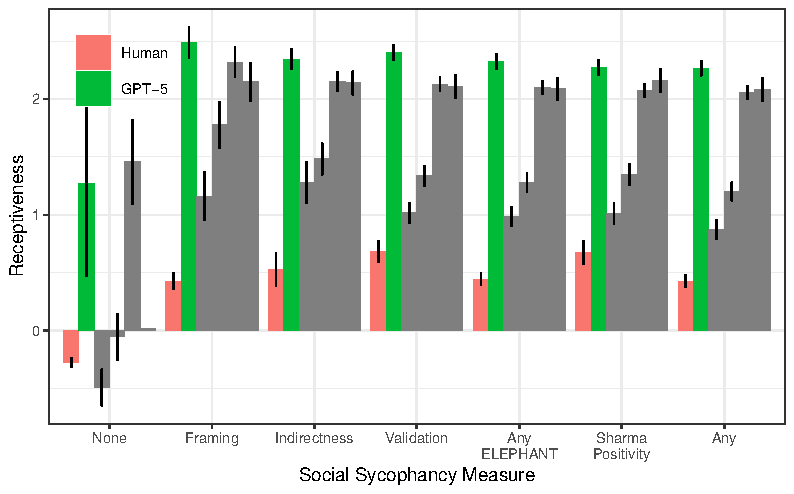
\includegraphics[width=0.7\textwidth]{Figures/corr.pdf}
\caption{Receptiveness by individual social-sycophancy indicator, for human
top comments and GPT-5. ``None'' is responses triggering no indicator; ``Any
ELEPHANT'' pools validation, indirectness, and framing; ``Sharma positivity''
is the feedback-positivity indicator. Bars are $\pm2$ standard errors. Every
indicator is associated with higher receptiveness.}
\label{fig:corr_app}
\end{figure*}

\begin{figure*}[t]
\centering
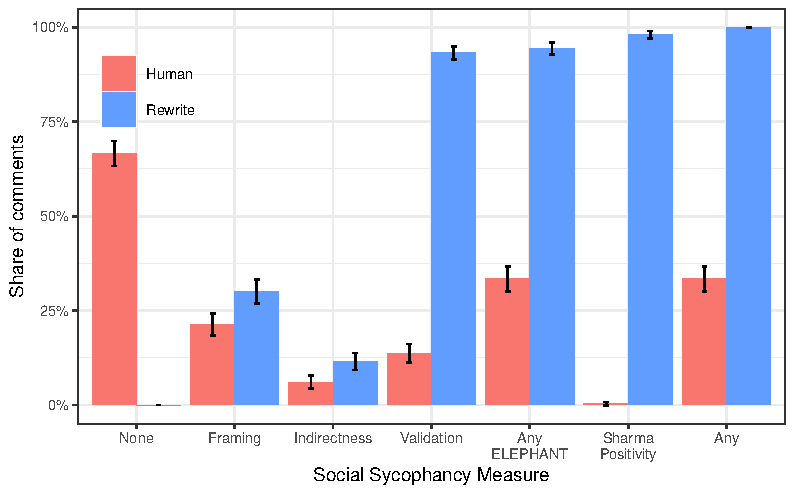
\includegraphics[width=0.7\textwidth]{Figures/shift.pdf}
\caption{Share of comments triggering each social-sycophancy indicator, before
and after the receptiveness-increasing rewrite. Bars are $\pm2$ standard
errors. Per-indicator decomposition of main-text Figure~2.}
\label{fig:shift_app}
\end{figure*}

\begin{figure*}[t]
\centering
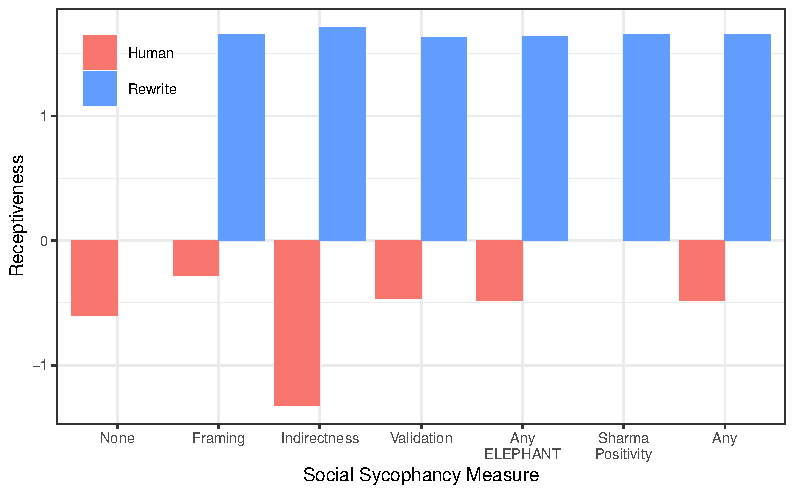
\includegraphics[width=0.7\textwidth]{Figures/shift_survey_n20.pdf}
\caption{Receptiveness by social-sycophancy indicator, restricted to the 100
scenarios used in the experiment. The experimental subsample behaves like the
full corpus.}
\label{fig:shift_survey}
\end{figure*}

\subsection{Experimental outcomes in full}

\needs{One paragraph: the main text reports summary statistics for quality and
the two preference items; these figures give the full distributions and the
splits by the participant's own verdict.}

\begin{figure}[t]
\centering
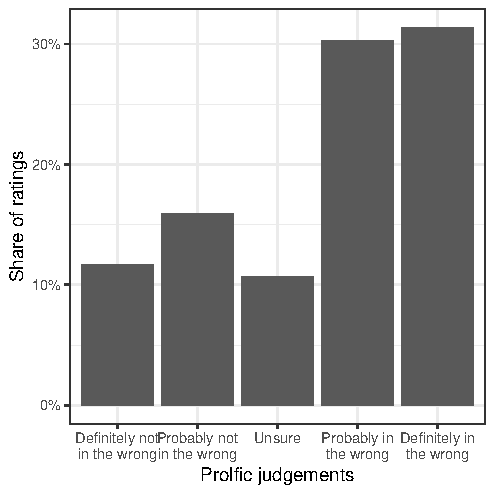
\includegraphics[width=\columnwidth]{Figures/verdicts_dist.pdf}
\caption{Distribution of participants' own verdicts on the experimental items.
Although every item is drawn from the AITA-YTA slice, where both the Reddit top
comment and the models judged the asker to be in the wrong, participants judged
the asker not to be in the wrong on 27.6\% of ratings (95\% CI [24.8\%,
30.5\%]).}
\label{fig:verdicts}
\end{figure}

\begin{figure*}[t]
\centering
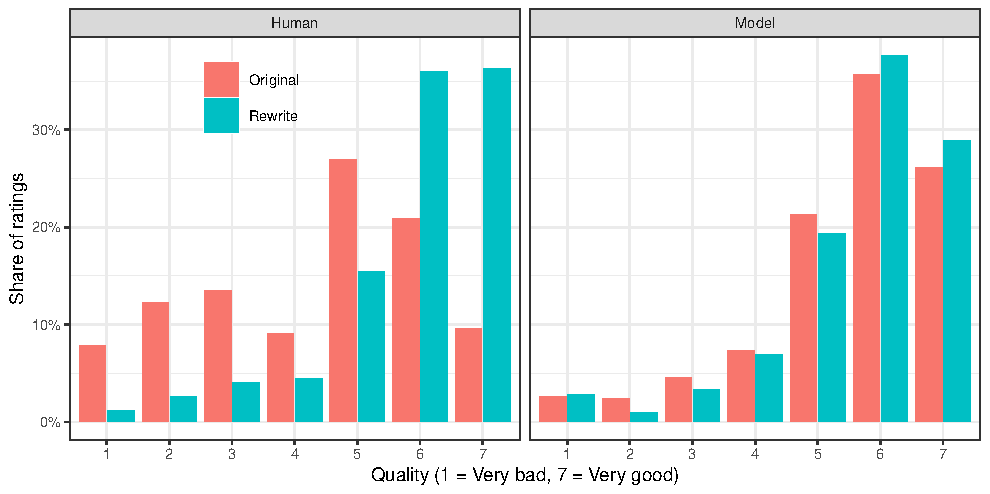
\includegraphics[width=0.7\textwidth]{Figures/advice_quality_dist.pdf}
\caption{Full distribution of seven-point quality ratings for the original
response and its receptive rewrite, faceted by whether the original was a human
top comment or a model generation.}
\label{fig:qual_dist}
\end{figure*}

\begin{figure*}[t]
\centering
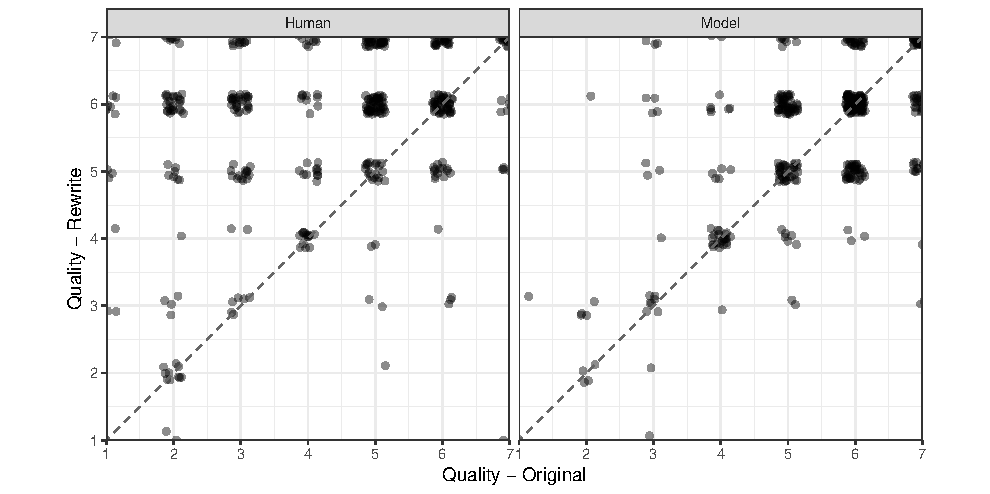
\includegraphics[width=0.7\textwidth]{Figures/advice_quality_scatter.pdf}
\caption{Paired quality ratings, rewrite against original, faceted by
provenance. Points above the diagonal are ratings on which the participant
preferred the rewrite.}
\label{fig:qual_scatter}
\end{figure*}

\begin{figure*}[t]
\centering
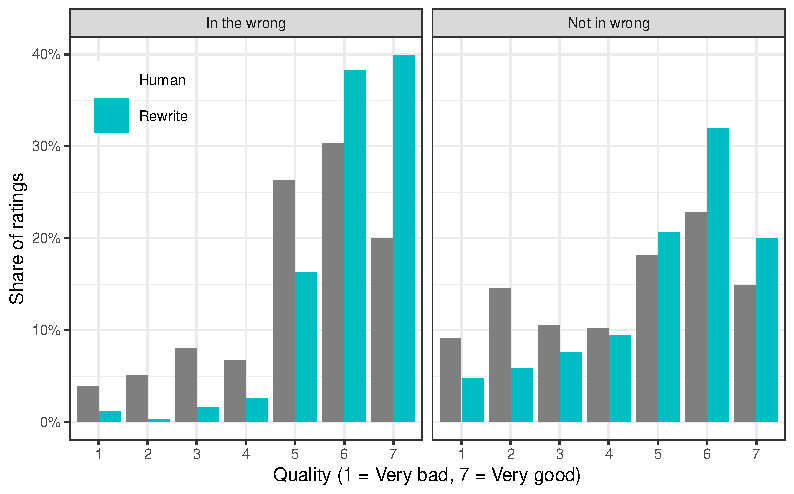
\includegraphics[width=0.7\textwidth]{Figures/quality_by_verdict.pdf}
\caption{Quality ratings split by the participant's own verdict on the case.
The rewrite is rated higher whether or not the participant judged the asker to
be in the wrong, so the preference is not confined to participants sympathetic
to the asker.}
\label{fig:qual_verdict}
\end{figure*}

\needs{Decide whether the two preference-by-verdict panels
(\texttt{advice\_listen.pdf}, \texttt{advice\_personal.pdf}) belong here as
well. See the note below before including them.}

\todo{In \texttt{analysis.R}, the ggsave block under ``Pref share by verdict''
writes \texttt{p\_advice\_verdict} to \texttt{advice\_personal.pdf} but writes
\texttt{p\_listen}---the main-text Figure~4 panel---to
\texttt{advice\_listen.pdf}, rather than \texttt{p\_listen\_verdict}. The
listen-by-verdict figure is therefore never saved. Fix before including either
panel here.}

\subsection{Item-level heterogeneity}

\needs{One paragraph: main-text Figure~3 shows the preference gap shrinking as
the original becomes more receptive; this figure shows the same heterogeneity
on the quality outcome, item by item.}

\begin{figure*}[t]
\centering
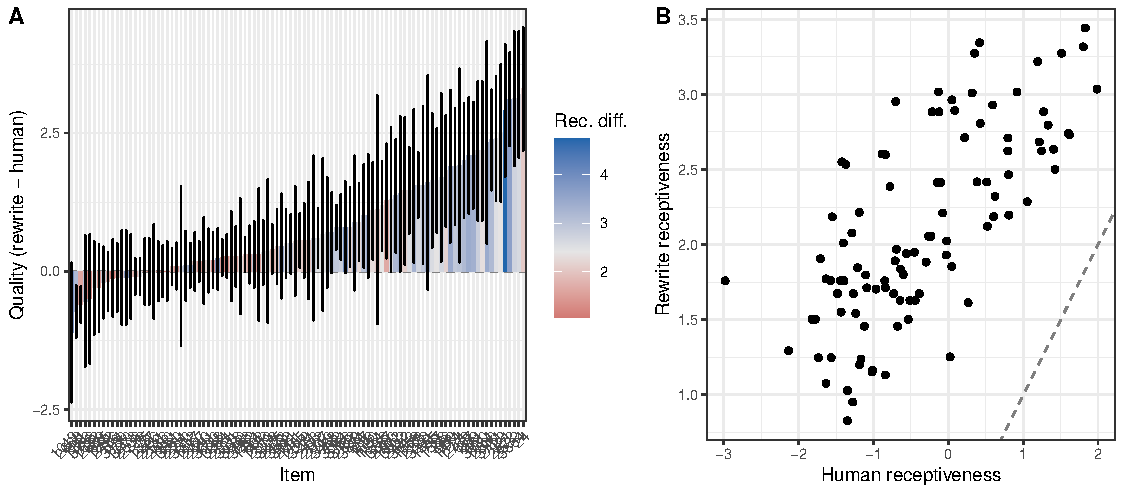
\includegraphics[width=0.9\textwidth]{Figures/advice_delta_by_item.pdf}
\caption{(A) Per-item quality difference, rewrite minus original, ordered by
effect size and shaded by the item's receptiveness gain. Bars are $\pm2$
standard errors. (B) Receptiveness of each item's rewrite against that of its
original; all items lie above the diagonal, since items were selected to gain
at least one standard deviation.}
\label{fig:deltas}
\end{figure*}

% ===========================================================================
% References
% ===========================================================================
% Same convention as the main text: no hand-written BibTeX.

\bibliography{receptiveness}

\end{document}
